\documentclass[conference]{IEEEtran}
\usepackage[T1]{fontenc}
\usepackage{graphicx,booktabs,amsmath,cite,url}
\usepackage[hidelinks]{hyperref}

\begin{document}

\title{MQTT, CoAP and HTTP Under Constrained Networks: A Reproducible Benchmark with JSON and CBOR Encodings}

\author{\IEEEauthorblockN{<<AUTHOR>>}
\IEEEauthorblockA{Independent Researcher<<EMAIL_LINE>>}}

\maketitle

\begin{abstract}
IoT devices often communicate over slow, lossy links, yet protocol comparisons are frequently run on clean networks. We present a reproducible benchmark of MQTT, CoAP and HTTP with JSON and CBOR payloads under five emulated network profiles (baseline, 4G-like, 3G-like, 2G-like and 10\% loss). Across 18,000 measured messages (three repetitions per configuration, plus 3,600 calibration messages), all three protocols delivered every message, but their costs differed sharply. CoAP needed <<coap_b>> bytes on the wire per message versus <<http_b>> for HTTP (<<ratio_b>>$\times$ less) and tracked the link's one-way delay most closely. With 10\% packet loss, however, CoAP's fixed 2--3\,s retransmission timer produced a 95th-percentile latency of <<l_coap_p95_ms>>\,ms, compared with <<l_http_p95>>\,ms for HTTP and <<l_mqtt_p95>>\,ms for MQTT, and 7 of 1,200 CoAP messages were delivered but never acknowledged within 15\,s. CBOR reduced payload size by 18\% but total traffic by only <<cbor_http>>--<<cbor_coap>>\%. We also document configuration pitfalls, including missing keep-alive, split writes interacting with Nagle's algorithm, and host-side emulation artifacts, which initially made HTTP appear about four times slower than it is. Code and data are released.
\end{abstract}

\begin{IEEEkeywords}
Internet of Things, MQTT, CoAP, HTTP, CBOR, network emulation, benchmarking
\end{IEEEkeywords}

\section{Introduction}
Many IoT deployments, such as agricultural sensors, utility meters and environmental monitors, rely on cellular links with high latency, limited bandwidth and packet loss. Choosing an application protocol for such devices is a practical decision with consequences for latency, data cost and energy. The three most common choices are MQTT~\cite{mqtt311}, a publish/subscribe protocol over TCP with a broker; CoAP~\cite{rfc7252}, a REST-style protocol over UDP with optional confirmable messages; and HTTP/1.1~\cite{rfc9112}.

Earlier comparisons~\cite{thangavel2014,naik2017,gundogan2018} established that the protocols trade reliability against overhead differently. We contribute: (i) a fully scripted benchmark that runs on a single Linux machine and emulates network impairments at the packet level; (ii) measurements of latency, tail latency, delivery, bytes on the wire and receiver CPU for the three protocols with JSON~\cite{rfc8259} and CBOR~\cite{rfc8949} payloads under five network profiles; and (iii) a documented set of configuration and measurement pitfalls that can distort such comparisons by large factors.

\section{Related Work}
Thangavel et al.~\cite{thangavel2014} compared MQTT and CoAP through a common middleware and found that MQTT had lower delay at low loss rates but higher delay than CoAP at high loss rates, while CoAP generated less extra traffic for small messages. Naik~\cite{naik2017} compared MQTT, CoAP, AMQP and HTTP qualitatively across criteria such as message size, overhead and quality of service. G{\"u}ndo{\u{g}}an et al.~\cite{gundogan2018} measured NDN, CoAP and MQTT on constrained IoT hardware. Our work complements these studies with an emulated-profile methodology, payload-encoding comparisons, tail-latency analysis and an explicit account of measurement pitfalls.

\section{Testbed and Method}
\subsection{Protocol configurations}
Each protocol has a simulated sensor node that sends 200 readings (temperature, humidity, PM2.5, battery voltage; about 107 bytes in JSON) sequentially, with 50\,ms between messages. \textbf{HTTP}: a Flask application served by waitress~\cite{waitress}, one persistent keep-alive connection, \texttt{TCP\_NODELAY} on both ends, and each request sent in a single write. \textbf{CoAP}: aiocoap~\cite{aiocoap} with confirmable POST requests and default RFC~7252 transmission parameters. \textbf{MQTT}: a Mosquitto~2.0 broker~\cite{light2017} and paho-mqtt clients~\cite{paho} at QoS~1, with \texttt{TCP\_NODELAY} on clients and broker. The receiver subscribes before measurement starts and signals readiness only after the broker confirms the subscription.

\subsection{Network emulation}
Impairments are applied to the benchmark ports on the loopback interface by a userspace emulator built on Linux NFQUEUE, used because the test kernel lacks \texttt{netem}~\cite{hemminger2005}. It applies normally distributed delay jitter, random loss and a rate limit on a single FIFO queue that never reorders packets. Like \texttt{netem} on loopback, it impairs both directions, so the round-trip delay is about twice the configured delay. Table~\ref{tab:profiles} lists the profiles. They are illustrative approximations of typical mobile conditions, not measurements of a specific operator. A calibration profile with the emulator active and zero delay added only 0.18--0.23\,ms to median latency.

\begin{table}[t]
\caption{Emulated network profiles (applied in each direction).}
\label{tab:profiles}
\centering\footnotesize
\begin{tabular}{@{}lccc@{}}
\toprule
Profile & Delay (jitter) & Loss & Rate \\
\midrule
Baseline & -- & -- & -- \\
4G-like & 25\,ms ($\pm$5) & 0.5\% & -- \\
3G-like & 100\,ms ($\pm$20) & 1.5\% & 1\,Mbit/s \\
2G-like & 250\,ms ($\pm$50) & 3\% & 100\,kbit/s \\
Lossy & 10\,ms & 10\% & -- \\
\bottomrule
\end{tabular}
\end{table}

\subsection{Metrics}
\emph{One-way latency}: the sender embeds a timestamp, and the receiver subtracts it on arrival (sender and receiver share a clock). For MQTT this spans sensor $\rightarrow$ broker $\rightarrow$ subscriber. \emph{RTT}: from send to the protocol-level acknowledgment (HTTP response, CoAP ACK, MQTT PUBACK from the broker). \emph{Delivery}: unique message IDs received divided by those sent. \emph{Bytes on the wire}: change in the loopback interface's transmitted-byte counter during a run divided by the number of messages, including headers, TCP acknowledgments and retransmissions. For MQTT this counts both hops. \emph{Receiver cost}: CPU time and peak resident memory of the receiving processes (broker plus subscriber for MQTT). Each configuration (5 profiles $\times$ 3 protocols $\times$ 2 encodings) ran three times. The host had 4 vCPUs (Intel Xeon, 2.8\,GHz) and ran Linux~6.18 and Python~3.13.

\section{Measurement Pitfalls}\label{sec:pitfalls}
The first version of the benchmark reported a median HTTP latency of about 440\,ms on the 3G-like profile, four times the link delay. Packet captures revealed three causes, none inherent to HTTP. First, Flask's development server closes the connection after every response, adding a TCP handshake to each message. Second, the \texttt{requests} library writes headers and body separately, and Nagle's algorithm~\cite{rfc896} then delays the body by one round trip until the headers are acknowledged. Third, because the emulator delays packets on the sending host, Linux TCP autocorking held small writes while an earlier packet was still queued locally, which would not happen on a real network. We disable autocorking during emulated runs. After these fixes, HTTP's median on the same profile was <<g3_http>>\,ms.

Two further issues affected individual runs. Downloads made through a localhost proxy during the benchmark inflated the loopback byte counter, so every run that overlapped such activity was discarded and repeated. A receiver that announced readiness before its MQTT subscription was confirmed lost the first message in one lossy run; the receiver was fixed and all lossy MQTT runs were repeated. Both sets of superseded data are released alongside the final results. We recommend that protocol benchmarks report connection reuse, \texttt{TCP\_NODELAY} settings and the location of emulation.

\section{Results}
\subsection{Baseline and bytes on the wire}
On the unimpaired baseline, median one-way latency was <<b_mqtt>>\,ms (MQTT), <<b_http>>\,ms (HTTP) and <<b_coap>>\,ms (CoAP), so the protocol barely matters on a good network. Overheads differ substantially (Fig.~\ref{fig:bytes}). CoAP required about <<coap_b>> bytes per message (one request and one acknowledgment datagram), HTTP about <<http_b>> and MQTT about <<mqtt_b>>. MQTT's figure covers two TCP hops, so per hop it is a little over half of HTTP's.

\begin{figure}[t]
\centering
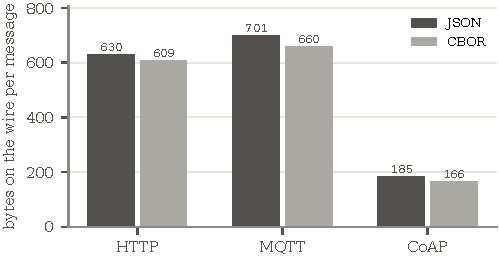
\includegraphics[width=\columnwidth]{figs/fig_bytes.pdf}
\caption{Bytes on the wire per message on the baseline profile, including headers and acknowledgments (MQTT includes both broker hops).}
\label{fig:bytes}
\end{figure}

\begin{figure*}[t]
\centering
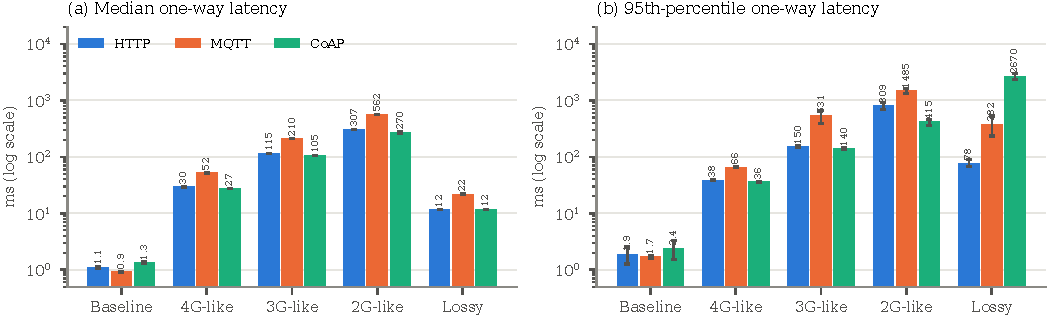
\includegraphics[width=\textwidth]{figs/fig_latency.pdf}
\caption{One-way latency with JSON payloads (mean over three repetitions, error bars show standard deviation; log scale). MQTT latency includes the broker hop.}
\label{fig:lat}
\end{figure*}

\subsection{Latency on constrained links}
Fig.~\ref{fig:lat}(a) and Table~\ref{tab:results} show that CoAP and HTTP medians follow the link's one-way delay: on the 4G-, 3G- and 2G-like profiles CoAP took <<g4_coap>>, <<g3_coap>> and <<g2_coap>>\,ms, and HTTP took <<g4_http>>, <<g3_http>> and <<g2_http>>\,ms. The HTTP--CoAP gap grows from about <<gap4>>\,ms to <<gap2>>\,ms as the link worsens, plausibly because TCP acknowledgments queue ahead of data on the jittered link. MQTT took roughly twice as long (<<g4_mqtt>>, <<g3_mqtt>> and <<g2_mqtt>>\,ms) because both hops crossed the impaired link in our topology. The sender's wait for the broker's acknowledgment was similar to the other protocols (median RTT <<g4_mqtt_rtt>>\,ms versus <<g4_coap_rtt>>\,ms for CoAP on 4G-like), so in deployments where the broker sits next to the consumers, the second hop is short.

\begin{table}[t]
\caption{Results with JSON payloads (means over three repetitions).}
\label{tab:results}
\centering\footnotesize\setlength{\tabcolsep}{3.5pt}
\begin{tabular}{@{}llrrrr@{}}
\toprule
Profile & Protocol & Median & p95 & Median RTT & Bytes/ \\
 & & (ms) & (ms) & (ms) & msg \\
\midrule
<<TABLE_RESULTS>>
\bottomrule
\end{tabular}
\end{table}

\subsection{Packet loss and retransmission}
All protocols delivered 100\% of messages on every profile, because each provides reliability (TCP retransmission, CoAP confirmable messages, MQTT QoS~1). Loss therefore appears as delay. With 10\% loss, medians stayed near the link delay, but the 95th percentile was <<l_http_p95>>\,ms for HTTP, <<l_mqtt_p95>>\,ms for MQTT and <<l_coap_p95_ms>>\,ms for CoAP (Fig.~\ref{fig:lat}(b)). Linux TCP adapts its retransmission timing to the measured round-trip time and uses tail-loss probes~\cite{rfc6298,rfc8985}, so a lost segment on this 20\,ms path is typically recovered within tens of milliseconds. CoAP's default initial timeout is 2--3\,s regardless of the path~\cite{rfc7252}. In addition, 7 of the 1,200 CoAP messages on this profile reached the receiver but were never acknowledged to the sender within 15\,s, so a real device would have treated them as failed. On the 2G-like profile (3\% loss), in contrast, CoAP had the lowest 95th percentile (<<g2p95_coap>>\,ms versus <<g2p95_http>>\,ms for HTTP and <<g2p95_mqtt>>\,ms for MQTT), because fewer than 5\% of messages needed a retransmission. On that profile, however, CoAP senders waited up to about <<g2_coap_rtt_p95>>\,s (95th-percentile RTT) for acknowledgments that had been lost. Tail latency on the 2G-like profile also varied considerably between repetitions.

\subsection{JSON versus CBOR}
CBOR reduced the payload from about 108 to 89 bytes ($-$18\%). Total bytes on the wire fell by <<cbor_coap>>\% for CoAP, <<cbor_mqtt>>\% for MQTT and <<cbor_http>>\% for HTTP, since headers and acknowledgments dominate small messages. CBOR had no consistent effect on latency.

\subsection{Receiver cost}
Receiver CPU per message was about <<cpu_mqtt>>\,ms for MQTT (C broker plus Python subscriber), <<cpu_coap>>\,ms for CoAP and <<cpu_http>>\,ms for HTTP, with peak memory of <<mem_mqtt>>, <<mem_coap>> and <<mem_http>>\,MB. These numbers reflect the specific implementations rather than the protocols themselves.

\section{Discussion and Limitations}
For battery- or data-constrained devices on poor links, CoAP minimizes bytes and median latency, but its retransmission parameters should be tuned where loss is common. MQTT suits fan-out to many consumers, and broker placement determines its latency. HTTP is competitive once connections are reused and requests are sent in a single write. CBOR is most useful where protocol overhead is already small, as with CoAP.

All measurements used one machine, loopback networking and emulated impairments rather than radios or operator networks, and impairments were applied at the sending host. Messages were small and sent one at a time, so throughput effects of larger transfers were not studied. Implementations were Python-based (except Mosquitto) rather than embedded firmware.

\section{Conclusion}
Under constrained networks, CoAP is the leanest protocol and the fastest in the median, HTTP is close behind when configured correctly, and MQTT's latency depends on broker placement. Under heavy loss, CoAP's default retransmission timer dominates its tail latency. Above all, configuration details can shift protocol comparisons by factors of four, so benchmarks should report them.

\section*{Data Availability}
Code, raw data and the network emulator are available <<REPO_URL>>.

\section*{Acknowledgment}
The author used Claude (Anthropic), an AI assistant, to help write the benchmark code, run the experiments and draft this manuscript. The author is responsible for the content of the paper.

\bibliographystyle{IEEEtran}
\bibliography{refs}

\end{document}
